\section{Model Architecture}
\label{sec:model}

Amphion EmoAnalyzer consists of three components: (i)~a frozen audio encoder that maps a 16\,kHz waveform into continuous speech representations, (ii)~a trainable two-layer adapter that projects the encoder's output into the LLM's embedding space, and (iii)~a LoRA-tuned 1.5B-parameter LLM decoder that generates categorical SER labels and free-form DEA narratives from a shared speech-language input sequence. \Cref{fig:model_arch} illustrates the overall architecture and the training state of each component.

The three-stage design reflects three concrete engineering constraints. \textit{First}, we freeze the audio encoder to prevent catastrophic forgetting of the acoustic representations acquired during large-scale pre-training; the relatively small volume of emotion-labeled speech ($\sim$1,000 hours) is insufficient to retrain an encoder without degrading its general acoustic quality. \textit{Second}, we introduce an explicit adapter module rather than projecting encoder outputs directly into the LLM embedding space: decoupling modality alignment from emotional reasoning allows the adapter to specialize in bridging acoustic and semantic feature spaces without entangling this with the LLM's optimization objective. \textit{Third}, we apply LoRA to the LLM backbone rather than full fine-tuning, because full-weight updates on domain-specific emotion data risk overfitting and degrading the broad language and instruction-following capability that makes open-form DEA generation possible.

% TODO: convert to TikZ figure using figures/_palette.tex (domain-constraints.mdc §9)
\begin{figure}[ht]
\centering
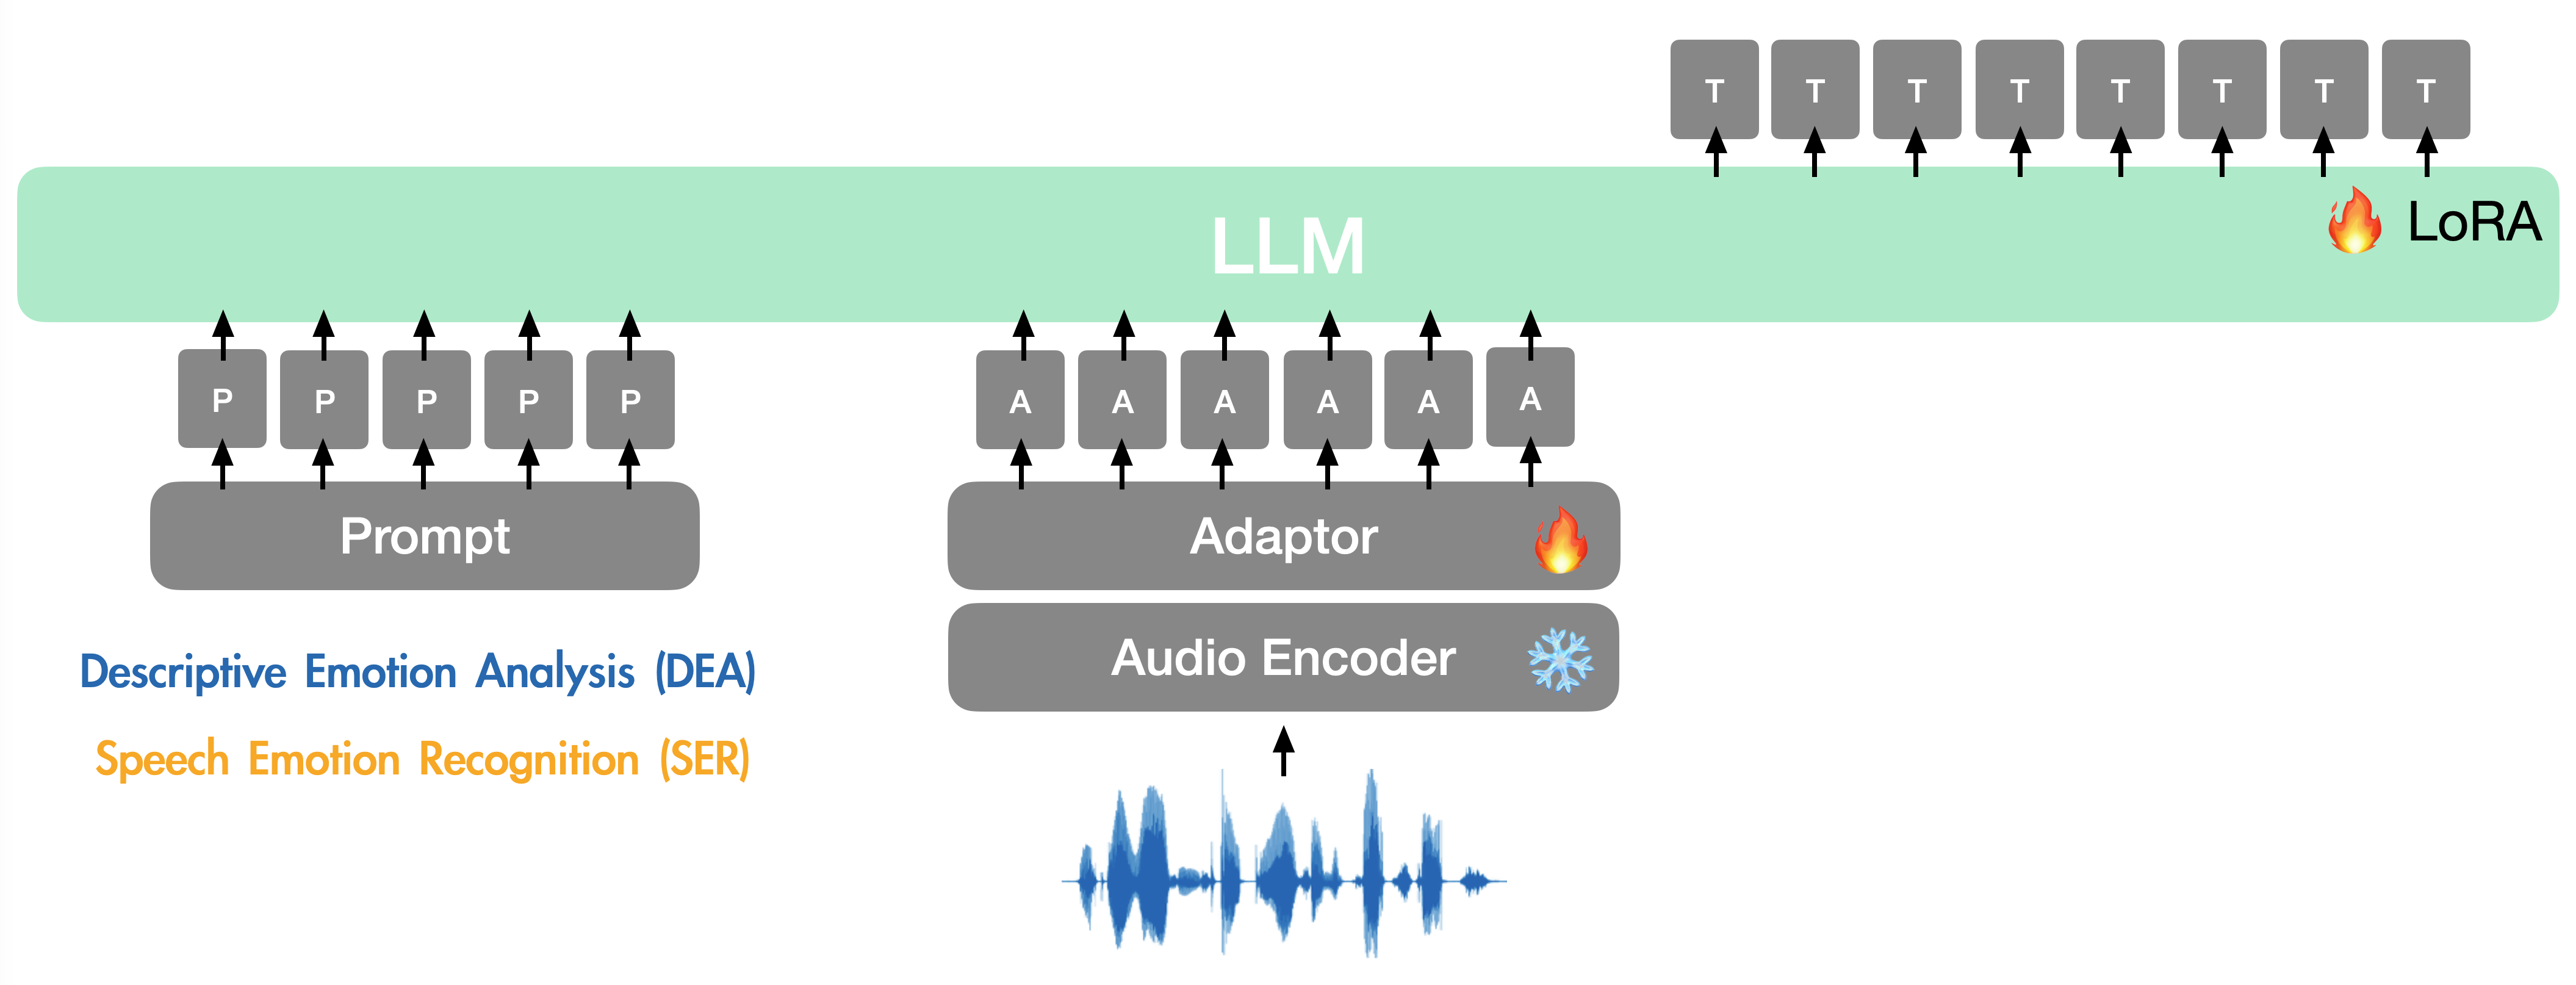
\includegraphics[width=0.8\columnwidth]{images/model_arch.png}
\caption{Overall architecture of Amphion EmoAnalyzer. The audio encoder (frozen) maps waveforms to speech representations; the adapter (trainable) bridges encoder and LLM embedding spaces; the LLM decoder (LoRA-tuned) generates SER labels and DEA narratives conditioned on the merged speech--text sequence.}
\label{fig:model_arch}
\end{figure}


\subsection{Audio Encoder}

The audio encoder is initialized from the AuT (Audio Tokenizer) encoder of the Qwen3-Omni-Captioner model \cite{qwen3omni-captioner}, a Whisper-style pre-LN Transformer that processes 16\,kHz mono audio through a log-mel front-end and a convolutional sub-sampler. To adapt the encoder for direct connection to our adapter, we omit its final two projection layers that originally mapped outputs to the Qwen3 LLM latent space. The encoder weights remain \textbf{frozen} throughout all training stages.

% TODO: add encoder architecture table (layers, hidden dim, attention heads, FFN dim, output frame rate, output dim)
% — verify against Qwen3-Omni-Captioner encoder checkpoint, NOT the Qwen3-ASR AuT config


\subsection{Adapter}

The adapter is a two-layer fully connected network that bridges the audio encoder output space and the LLM decoder input space. It is the primary trainable module alongside the LoRA parameters and remains trainable throughout all training stages.

% TODO: add adapter input/output dimensions and parameter count — verify against model config


\subsection{LLM Decoder}

The decoder is Qwen2.5-1.5B-Instruct \cite{qwen2.5}, a compact decoder-only Transformer chosen for its strong instruction-following capability at a parameter budget compatible with efficient joint training. During training, LoRA modules are injected into all linear projection layers within the attention mechanisms and feed-forward networks, while the base LLM weights remain frozen. The LoRA configuration uses a rank of $r{=}64$, a scaling factor of $\alpha{=}16$, and a dropout rate of $0.05$.

% TODO: add LLM architecture table (layers, hidden dim, attention heads, KV heads, FFN dim)
% — verify against Qwen2.5-1.5B-Instruct model config


\subsection{Task Prompt Templates}

EmoAnalyzer handles three tasks through a unified prompt interface. Each task is presented to the LLM as a short instruction line followed by an audio placeholder, which is replaced by the adapter-projected audio embedding sequence at the merge step. The same templates are used at both training and inference time.

% TODO: paste the literal prompt templates for SER / DEA / ASR (En and Zh)
% — verify against internal task_prompts config; do not paraphrase

At inference, the model produces a discrete emotion label for SER tasks and a natural-language narrative for DEA tasks, allowing both output formats to coexist within a single model without task-specific output heads.
